\documentclass[]{article}
\usepackage[T1]{fontenc}
\usepackage[utf8]{inputenc}
%\usepackage[icelandic]{babel}
\usepackage{caption}
\usepackage{circuitikz}
\usepackage{grffile} 
\usepackage[margin=1in]{geometry}

% grffile er pakki sem leifir manni að nota "" til þess að forðast að nota
% nafnið á myndinni með.
\usepackage{graphicx}
% \graphicspath{{images/}} Sýnir undir möppu þar sem myndirnar eru

\usepackage{hyperref}
%fyrirlinka - \url{www.....}
\begin{document}


\title{Heimadæmi  \\ Einstaklingsverkefni \\ Stærfræði og reiknifræði}
\author{Pétur Daníel Ámundason \\ \\ pda3@hi.is}
\maketitle

\section*{1.}

1. Dæmi 5.2 í bók.


Ef neminn sýnir framm á að 400 hlutabréfin(sem hefur 250 viðskipta daga) sé samsetninginn úr fullt af hlutabréfum óháðum GOOG. Með því að geima hvert hlutabréf í vector a1, ..., a400 þar sem hver vector hefur upplýsingar um hvern viðskipta dag x [x1,x2, ... , x250]. Nemminn reiknar úr gögnum og notar breituna $\beta$ til þess að tákna scalar. $\beta_{1}a_{1} + ... + \beta_{k}a_{k } = 0$ ef nemminn nær að sína framm á þetta hefur hann rétt fyrir sér. En það er mjög ólíklegt eins og yfirmaðurinn sagði.

\section*{2.}
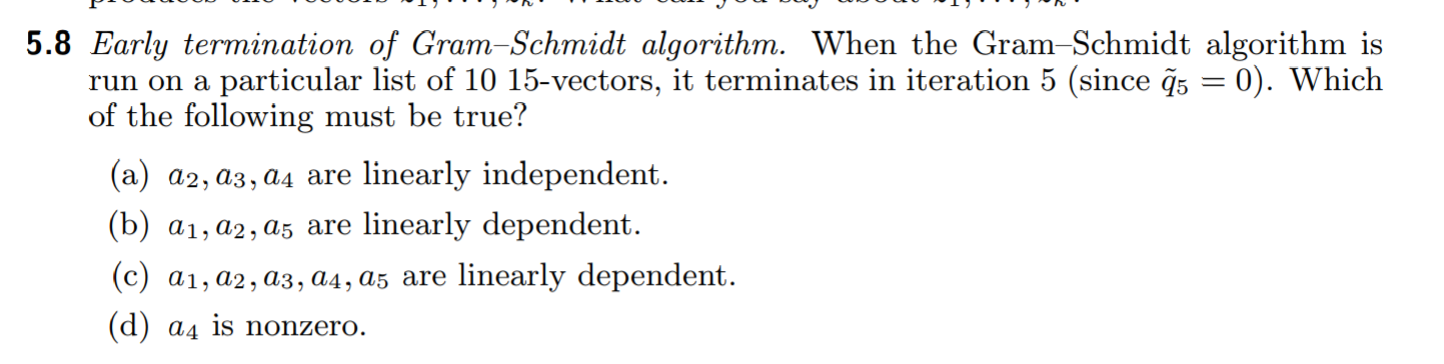
\includegraphics[scale=0.5]{d2}
svar c) \\
Ef reikniritið hættir í skrefi 2 þegar   $\tilde{q}_{5}$ = 0 þá er upphaflega safn af vektorum línulega háðir(linear dependant).

\section*{3.}
Til þess að velja lög fyrir notanda þá er athugað lagalistan sem hann hefur hlustað á og hvar hann er næstur miðpunktinum k.Svo er valið lög í kringum miðpunktinn í þeirri þyrpingu sem notandi hefur verið að hlusta lög sín í.

\section*{4.}





\end{document}